%!TEX root = ../thesis.tex
% ******************************* Thesis Appendix A ****************************


\ifpdf
\graphicspath{{Appendix1/Figs/Raster/}{Appendix1/Figs/PDF/}{Appendix1/Figs/}}
\else
\graphicspath{{Appendix1/Figs/Vector/}{Appendix1/Figs/}}
\fi

\chapter{Data quality and errors} 
\section{Tracking quality}
\label{sec:data_errors}
\begin{figure}[p]
    \centering
        \centering
        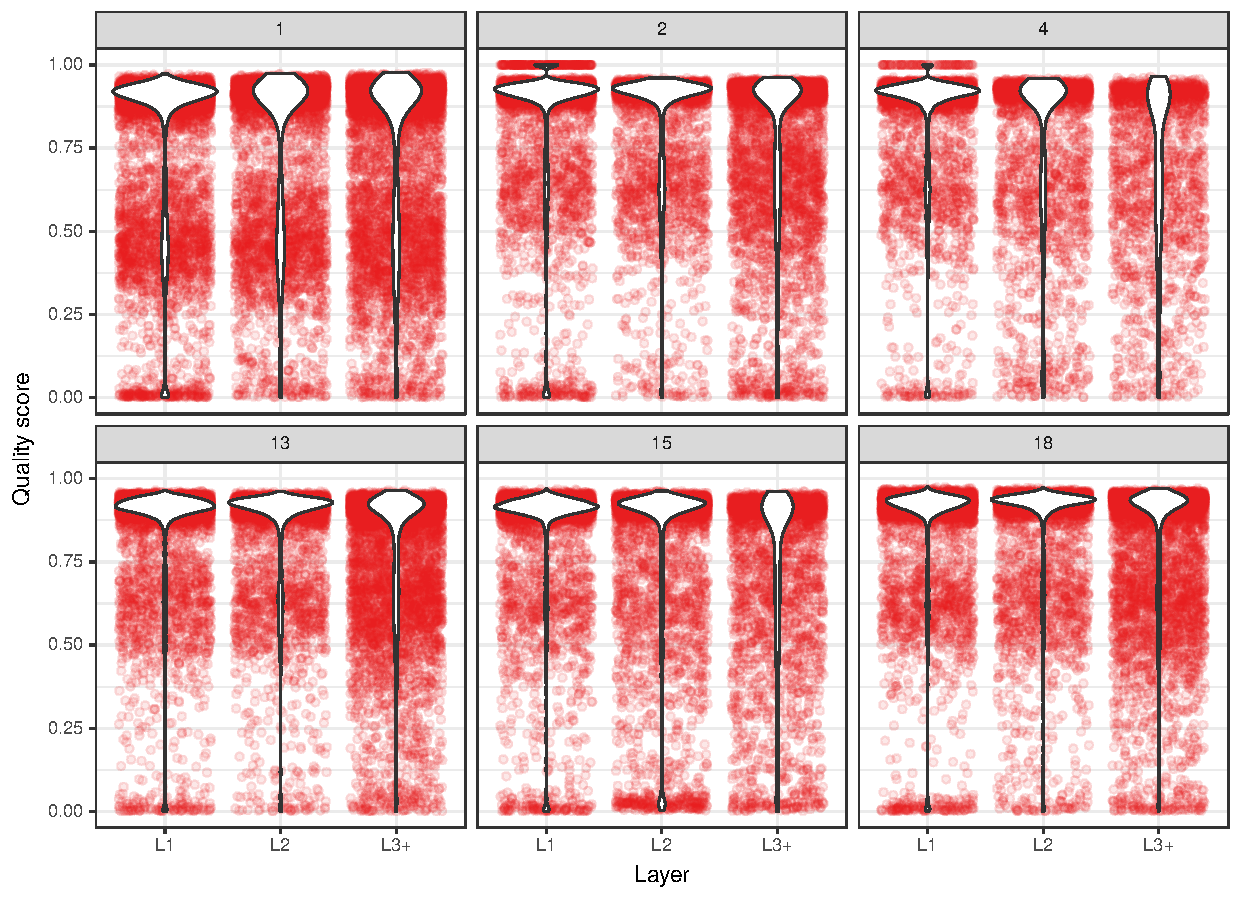
\includegraphics[width=.95\textwidth]{tracking_quality_layer.pdf}
        \centering
        \includegraphics[width=.95\textwidth]{tracking_quality_time.pdf} % second figure itself
        \caption[Tracking quality]{Quality distributions per plant, layer, and timepoint
          for all plants.
        Some timepoints have distributions scoring in the $\sim$1 regime, which
        corresponds to situations where the automatic tracking failed. These
        timepoints have been manually tracked for cells in the L1 within 30
        $\mu$m of the topmost CLV3 expressing cell.}
      \label{fig:tracking_quality}
\end{figure}
The data tracking quality is defined as the F1 score, also known as the
Dice-S{\o}rensen score, between timepoints. The
F1 score gives an appreciation of the overall accuracy of a test on the form of
\begin{equation}
  F_1 = 2 \frac{precision\times recall}{precision + recall},
  \label{eq:f1}
\end{equation}
i.e.\ as the harmonic mean between precision and recall. It can also be
expressed on set form as 
\begin{equation}
  F_1 = 2 \frac{X_t \cap X_{t+1}}{X_t \cup X_{t+1}}
  \label{eq:f1_set}
\end{equation}
where $X_t$ denotes the set in question in timepoint $t$. In other words, the more cells are
contained between timepoints, the higher the F1 score.

As \cref{fig:tracking_quality} shows, the quality for the tracking is overall
relatively high, with only a few timepoints having bigger clusters with low F1
scores. These cells are however typically positioned at the periphery of the
SAM, at the very edges of the segmentation, and are therefore both of lesser
interest and importance for the dynamics of the stem cell niche. As described in
\cref{sec:filtering}, we have in all of our analyses excluded the tracking of
cells whose F1 scores are less than $0.30$. The errors in tracking occasionally
causes one cell to be recognized as more than two in the next timeframe. In
these cases, we choose the two daughter cells by order of tracking quality.

That timepoints 40 and 48 hours in plant 2, as well as timepoint 20 hours in
plant 4 have perfect F1 scores is due to the tracking procedure failing at
these points. The tracking has therefore been manually corrected for the cells
within $30\mu$m of the highest CLV3 expressing cell.

\section{Segmentation quality}
\label{sec:data_errors_segmentation}
While holding an overall excellent quality, the data contains several types
of segmentation errors. For both the  
nuclear and the membrane segmentation, this typically takes the form of basins
of attraction identified as either one when there in fact are multiple, or
multiple when there is in fact only one. In particular, this causes errors with
respect to the apprciation of membrane and nuclear volumes. It also indirectly
affects the tracking quality, as clumped cells in one timepoint can lead to an
erroneously identified division event in the next, in case the segmentation
becomes correct. 

Segmentation errors are however the most prevalent in the peripheral regions of
the SAM, and with deeper penetration into the tissue. Generally, the membrane
segmentation holds higher quality than the nuclear one, where the latter
degrades quickly after deeper penetration than the L2. The overall quality is
also decreasing with the distance from the apex, although to a minor extent in
the L1. 

\begin{figure}[H]
  \centering
  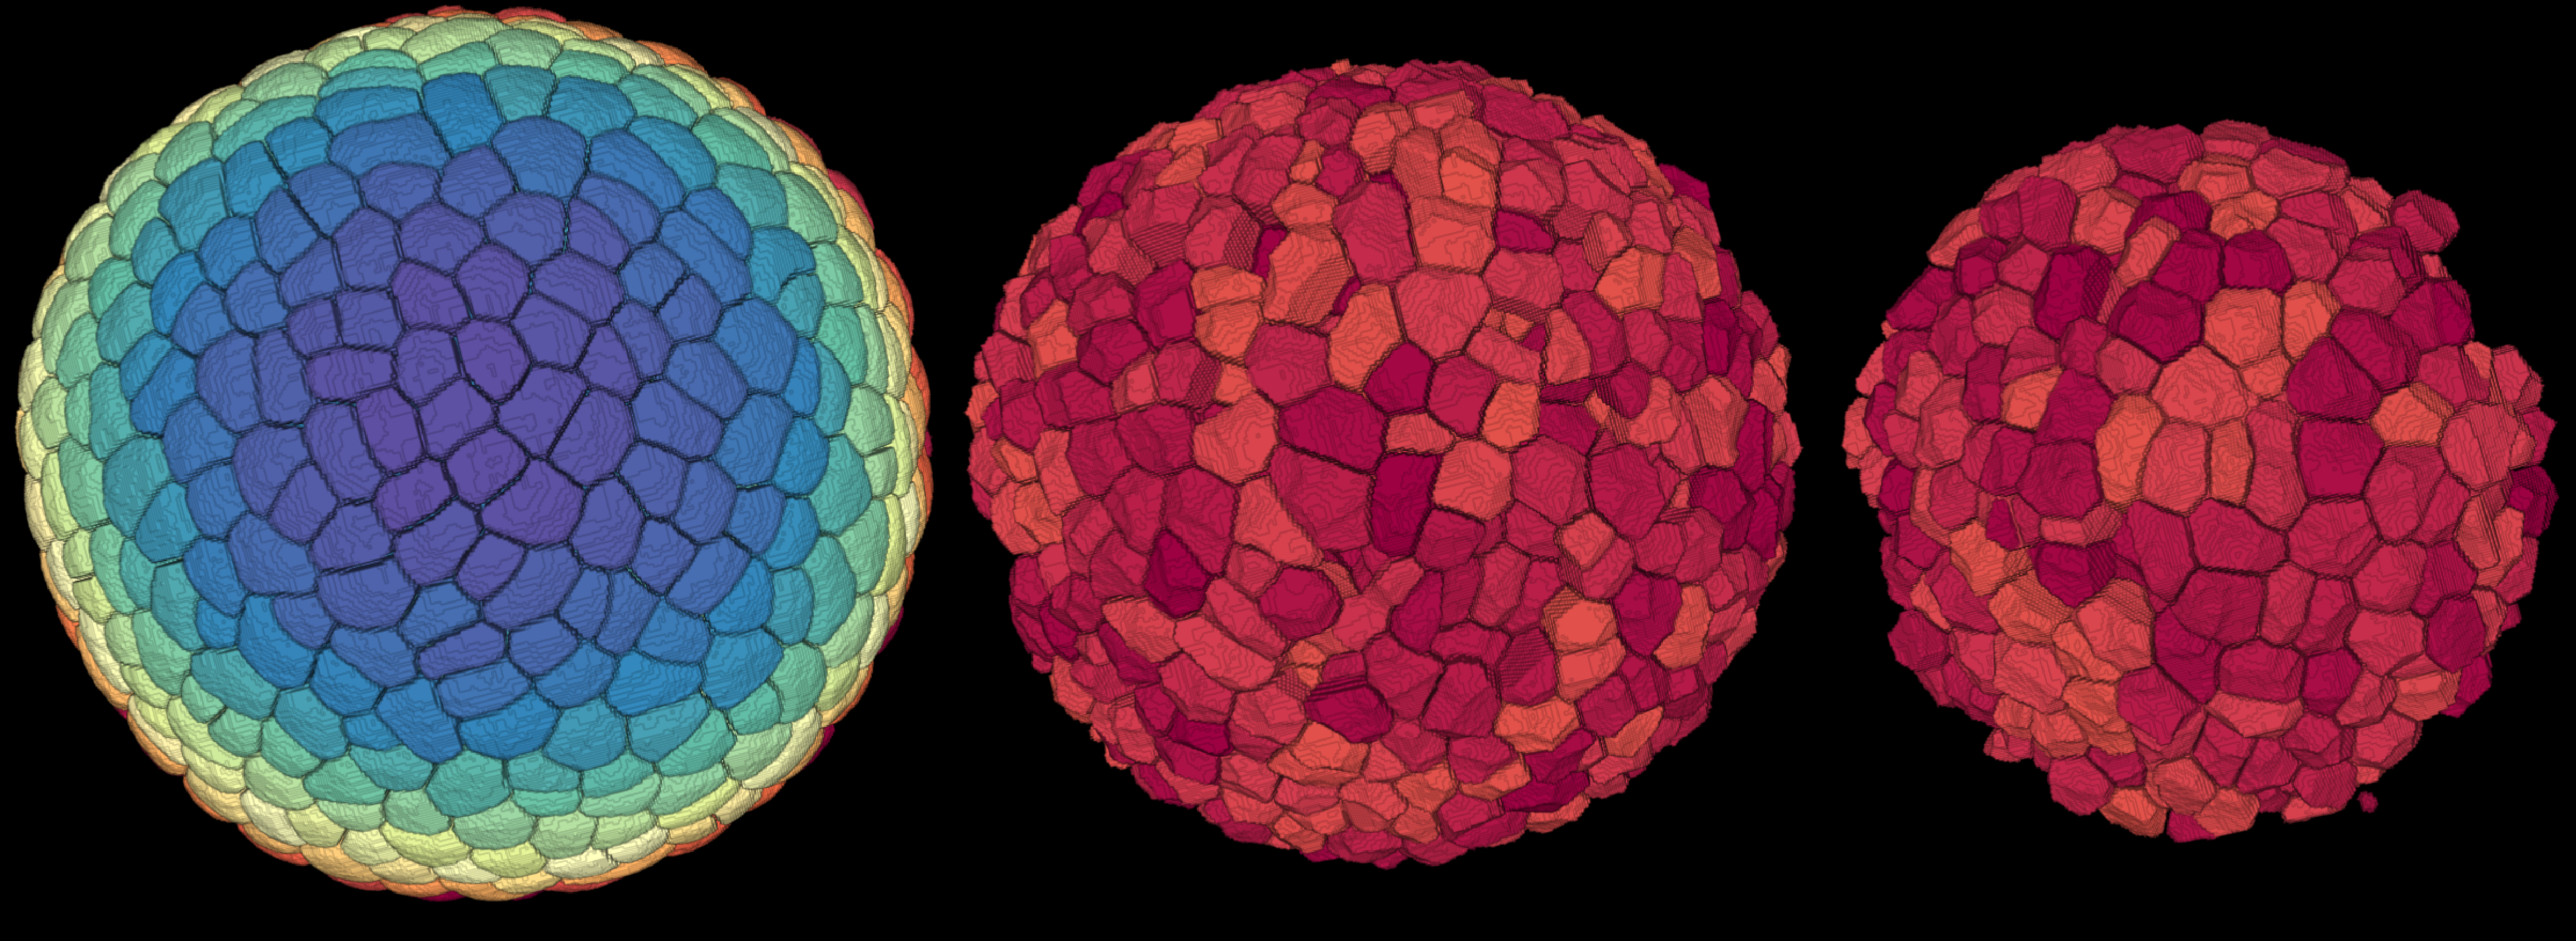
\includegraphics[width=\textwidth]{layer_quality_segm.pdf}
  \caption[Membrane segmentation quality per layer]{Membrane segmentation
    quality separated into L1, L2 and L3 respectively. L1 shows a smooth upper
    surface with well-segmented cells. Also L2 and L3 show high segmentation
    quality, but with a rougher surface to the cells being restricted by the
    cell layer on top, causing a ruggedness in the cell surface. Note in
    particular how the quality in the periphery of the SAM generally are of
    lesser quality, with occasional cell remnants being identified as actual
    cells, e.g.\ in the bottom right.}
  \label{fig:layer_quality_segm}
\end{figure}

Generally, the overall quality for the membrane segmentation is high in all
three layers, as shown in \cref{fig:layer_quality_segm}, although the number of errors increase with deeper tissue
penetration. For the nuclear segmentation, mostly cells from the L1 and L2 are
sufficiently reliable, with declining quality with larger distance to the CZ.
The errors with multiply matching nuclei are occurring mostly in the subepidermal
cells, and in those cases largely in the peripheral regions.

\section{Missing timepoints}
\label{sec:missingtp}
The dataset contains several missing timepoints in the nuclear and membrane
data. As previously noted, plant 1 and 18 lacks all timepoints for the nuclear
data, whereas plant 4 and 15 lack nuclear data for timepoints 24 and 12 hours
respectively. Plant 18 also lacks data for timepoint 40 hours.

